\section{RNA Secondary Structure \normalfont{\emoji{dna}}}

La ricerca della struttura secondaria dell'RNA è un problema a 2 variabili
risolvibile tramite il paradigma della programmazione dinamica. Come sappiamo il
DNA è composto da due filamenti, mentre l'RNA è composto da un filamento
singolo. Questo comporta che spesso le basi di un singolo filamento di RNA si
accoppino tra di loro. L'insieme della basi può essere visto come l'alfabeto
$\{A, C, U, G\}$ e l'RNA è una sequenza di simboli presi da questo alfabeto. Il
processo di accoppiamento delle basi è dettato dalla regola di \textit{Watson-Crick} e
segue il seguente schema:

\[
    A - U \ \ \ \textrm{ e } \ \ \ C - G \ \ \ \textrm{ (l'ordine non conta)}
\]

\begin{figure}[H]
    \centering
    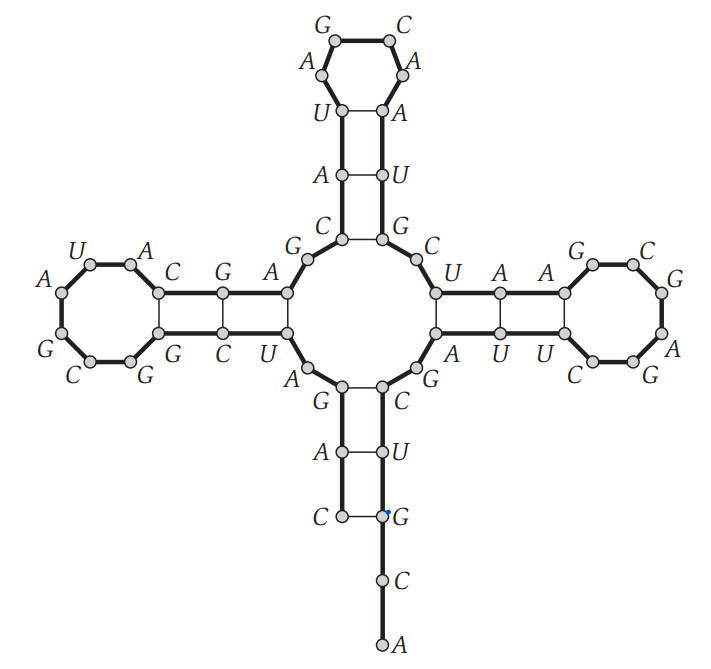
\includegraphics[width=8cm, keepaspectratio]{capitoli/dynamic_programming/imgs/rna_esempio1.png}
    \caption{Esempio di una struttura secondari di RNA} %%TODO: ricontrollare !!
\end{figure}

\subsection{Il Problema}

In questo problema si vuole trovare la struttura secondaria dell'RNA che abbia
energia libera maggiore (il maggior numero di coppie di basi possibili). Per
farlo dobbiamo tenere in considerazione alcune condizioni che devono essere
soddisfatte per permettere di approssimare al meglio il modello biologico
dell'RNA.\\

Formalmente la struttura secondaria di $B$ è un insieme di coppie $S =
    \{(i,j)\}$ dove $i,j \in \{1,2,\ldots,n\}$, che soddisfa le seguenti
condizioni:

\begin{enumerate}
    \item \textbf{No Sharp Turns}: la fine di ogni coppia è separata da almeno 4
          basi, quindi se $(i,j) \in S$ allora $i < j - 4$
    \item Gli elementi di una qualsiasi coppia $S$ consistono di $\{A, U\}$ o
          $\{C, G\}$ (in qualsiasi ordine).
    \item $S$ è un \textit{matching}: nessuna base compare in più di una coppia.
    \item \textbf{Non Crossing Condition}: se $(i, j)$ e $(k,l)$ sono due coppie
          in $S$ allora \textbf{non} può avvenire che $i < k < j < l$.
\end{enumerate}

\begin{figure}[H]
    \centering
    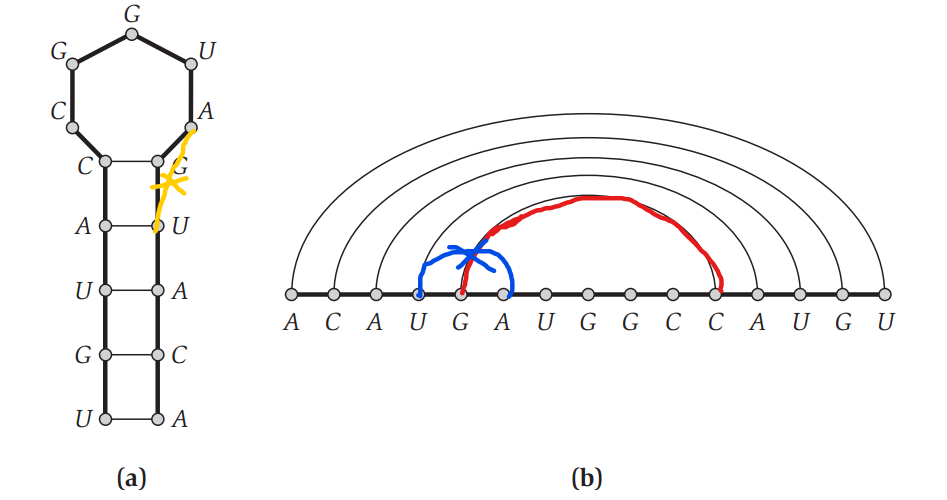
\includegraphics[width=10cm, keepaspectratio]{capitoli/dynamic_programming/imgs/rna_esempio2.png}
    \caption{La figura \textit{(a)} rappresenta un esempio di \textit{Sharp
            Turn}, mentre la figura \textit{(b)} mostra una
        \textit{Crossing Condition} dove il filo blu non dovrebbe esistere.}
\end{figure}

\subsection{\goal}

Il goal di questo problema è di massimizzare la quantità di coppie che si possono
formare all'interno della struttura secondaria di una data sequenza di RNA.

\subsection{Costi}

L'algoritmo complessivo ha costo $O(n^3)$.

\subsection{Funzionamento}

\paragraph{First Attempt.}
Come primo tentativo potremmo basarci sul seguente sotto-problema: affermiamo che
$OPT(j)$ è il massimo numero di coppie di basi sulla struttura secondaria $b_1
    b_2 \ldots b_j$, per la Non Sharp Turn Condition sappiamo che $OPT(j) = 0$ per
$j \leq 5$ e sappiamo anche che $OPT(n)$ è la soluzione che vogliamo trovare. Il
problema ora sta nell'esprimere $OPT(j)$ ricorsivamente. Possiamo parzialmente
farlo sfruttando le seguenti scelte:

\begin{itemize}
    \item $j$ non appartiene ad una coppia
    \item $j$ si accoppia con $t$ per qualche $t \leq
              j - 4$
\end{itemize}

Per il primo caso basta cercare la soluzione per $OPT(j - 1)$, nel secondo caso
invece se teniamo conto della Non Crossing Condition, possiamo isolare due nuovi
sotto-problemi: uno sulle basi $b_1 b_2 \ldots b_{t-1}$ e l'altro sulle basi
$b_{t+1} \ldots b_{j-1}$. Il primo si risolve con $OPT(t-1)$ ma il secondo, dato
che non inizia con indice $1$, non è nella lista dei nostri sotto-problemi. A
causa di ciò risulta necessario aggiungere una variabile.

\begin{figure}[H]
    \centering
    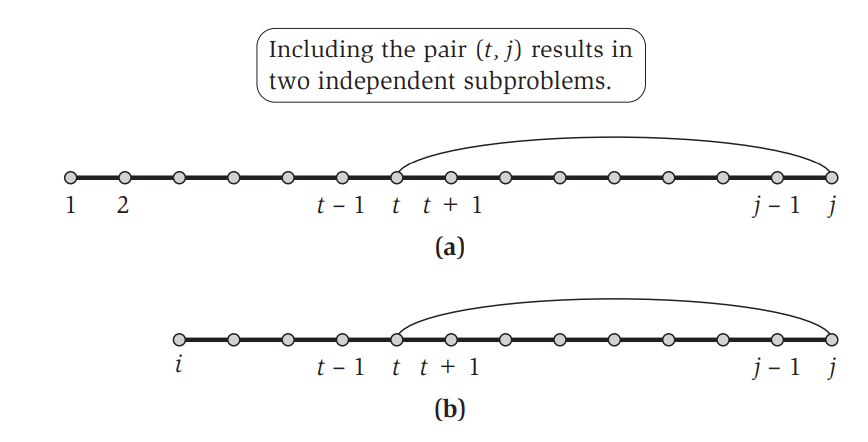
\includegraphics[width=10cm, keepaspectratio]{capitoli/dynamic_programming/imgs/rna_funzionamento.png}
    \caption{Esempio di
        utilizzo di una sola variabile \textit{(a)} o con due \textit{(b)}.}
\end{figure}

\paragraph{Dynamic Programming over Intervals}
Basandoci sui ragionamenti precedenti, possiamo scrivere una ricorsione di
successo: sia $OPT(i,j)$ il numero massimo di coppie di basi nella struttura
secondaria $b_i b_{i+1} \ldots b_j$, grazie alla non sharp turn Condition
possiamo inizializzare gli elementi con $i \geq j -4$ a $0$. Ora avremmo sempre
le stesse condizioni elencate sopra:

\begin{itemize}
    \item $j$ non appartiene ad una coppia
    \item $j$ si accoppia con $t$ per qualche $t \leq j - 4$
\end{itemize}

Nel primo caso avremmo che $OPT(i,j) = OPT(i, j-1)$, nel secondo caso possiamo
ricorrere su due sotto-problemi $OPT(i, t-1)$ e $OPT(t+1, j-1)$ affinché venga
rispettata la non crossing condition. Possiamo esprimere formalmente la
ricorsione come segue:

\begin{center}
    \[
        OPT(i, j) = \max(OPT(i, j-1), \max_t(1+OPT(i, t-1)+OPT(t+1, j-1))),
    \]
    dove il massimo è calcolato su $t$ tale che $b_t$ e $b_j$ siano una coppia di
    basi consentita
\end{center}

\begin{figure}[H]
    \centering
    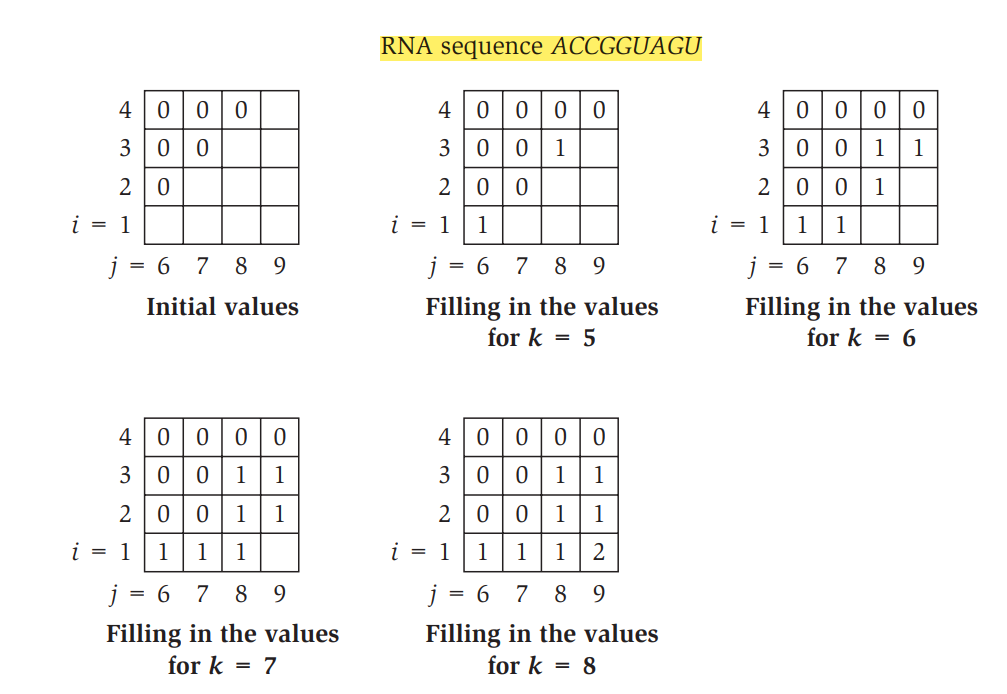
\includegraphics[width=\textwidth, keepaspectratio]{capitoli/dynamic_programming/imgs/rna_calcolo.png}
    \caption{Iterazioni dell'algoritmo su un campione del problema in questione $ACCGGUAGU$}
\end{figure}
\newpage

Possiamo infine formalizzare il tutto con il seguente pseudo-codice:

\begin{lstlisting}[language=JavaScript]
 Initialize OPT(i, j) = 0 whenever i ≥ j - 4

 for (k in 5 ... n - 1) {
     for (i in 1 ... n - k) {
         j = i + k
         Compute OPT(i, j) using the previous recurrence
     }
 }

 return OPT(1, n)
\end{lstlisting}

Ci sono $O(n^2)$ sotto-problemi da risolvere e ognuno richiede tempo $O(n)$,
quindi il running time complessivo è di $O(n^3)$.
